\chapter{R Package singleCellFeatures}
\label{app:singleCellFeatures}

Additional material. For example long mathematical derivations could be
given in the appendix. Or you could include part of your code that is
needed in printed form. You can add several Appendices to your thesis (as
you can include several chapters in the main part of your work).





\begin{rcode}
facetBorder <- function(x, y, img, facet) {
  facet.size <- img / facet
  # calculate facets (2d binning)
  x.bin <- ceiling(x / facet.size[1])
  y.bin <- ceiling(y / facet.size[2])
  # initialize empty grid/border matrices
  grid <- matrix(0, facet[2], facet[1])
  # calculate col-major grid index for each object
  index <- y.bin + (x.bin - 1) * facet[2]
  # summarize as counts
  counts <- table(index)
  # fill grid with counts
  grid[as.numeric(names(counts))] <- counts
  grid.res <- grid
  grid <- grid > 0
  # extend grid with a frame of ones
  grid.ext <- rbind(rep(1, (facet[1] + 2)),
                    cbind(rep(1, facet[2]), grid, rep(1, facet[2])),
                    rep(1, (facet[1] + 2)))
  # set up stencil
  row <- rep(rep(1:facet[2], facet[1]))
  col <- rep(1:facet[1], each=facet[2])
  colP1 <- col + 1
  colM1 <- col - 1
  rowP1 <- row + 1
  rowP2 <- row + 2
  nrowP <- facet[2] + 2
  stencil <- cbind(row   + colM1 * nrowP, # northwest neighbor
                   row   + col   * nrowP, # north neighbor
                   row   + colP1 * nrowP, # northeast neighbor
                   rowP1 + colP1 * nrowP, # west neighbor
                   rowP2 + colP1 * nrowP, # east neighbor
                   rowP2 + col   * nrowP, # southwest neighbor
                   rowP2 + colM1 * nrowP, # south neighbor
                   rowP1 + colM1 * nrowP) # southeast neighbor
  # apply stencil row-wise to grid
  border <- apply(stencil, 1, function(ind, mat) {
    return(sum(mat[ind]))
  }, as.numeric(grid.ext))
  # map col-major object index to border array
  return(border[index])
}
\end{rcode}


\begin{knitrout}\footnotesize
\definecolor{shadecolor}{rgb}{0.969, 0.969, 0.969}\color{fgcolor}\begin{kframe}
\begin{alltt}
\hlstd{edgepos} \hlkwb{<-} \hlkwa{function}\hlstd{(}\hlkwc{x}\hlstd{,} \hlkwc{y}\hlstd{,} \hlkwc{img}\hlstd{,} \hlkwc{n}\hlstd{) \{}
  \hlstd{empty} \hlkwb{<-} \hlkwd{logical}\hlstd{()}
  \hlstd{xst} \hlkwb{<-} \hlstd{img[}\hlnum{1}\hlstd{]} \hlopt{/} \hlstd{n}
  \hlstd{yst} \hlkwb{<-} \hlstd{img[}\hlnum{2}\hlstd{]} \hlopt{/} \hlstd{n}
  \hlstd{sgrid} \hlkwb{<-} \hlkwd{matrix}\hlstd{(}\hlnum{0}\hlstd{,} \hlkwc{nrow}\hlstd{=n,} \hlkwc{ncol}\hlstd{=n)}
  \hlkwa{for} \hlstd{(i} \hlkwa{in} \hlnum{1}\hlopt{:}\hlstd{n) \{}
    \hlkwa{for} \hlstd{(j} \hlkwa{in} \hlnum{1}\hlopt{:}\hlstd{n) \{}
      \hlstd{ispos} \hlkwb{<-} \hlstd{(x} \hlopt{>} \hlstd{(i} \hlopt{-} \hlnum{1}\hlstd{)} \hlopt{*} \hlstd{xst)} \hlopt{&} \hlstd{(x} \hlopt{<=} \hlstd{(i} \hlopt{*} \hlstd{xst))} \hlopt{&}
               \hlstd{(y} \hlopt{>} \hlstd{(j} \hlopt{-} \hlnum{1}\hlstd{)} \hlopt{*} \hlstd{yst)} \hlopt{&} \hlstd{(y} \hlopt{<=} \hlstd{(j} \hlopt{*} \hlstd{yst))}
      \hlstd{sgrid[i, j]} \hlkwb{<-} \hlkwd{sum}\hlstd{(ispos)}
    \hlstd{\}}
  \hlstd{\}}

  \hlkwa{for} \hlstd{(i} \hlkwa{in} \hlnum{1}\hlopt{:}\hlstd{n) \{}
    \hlkwa{for} \hlstd{(j} \hlkwa{in} \hlnum{1}\hlopt{:}\hlstd{n) \{}
      \hlstd{ispos} \hlkwb{<-} \hlstd{(x} \hlopt{>} \hlstd{(i} \hlopt{-} \hlnum{1}\hlstd{)} \hlopt{*} \hlstd{xst)} \hlopt{&} \hlstd{(x} \hlopt{<=} \hlstd{(i} \hlopt{*} \hlstd{xst))} \hlopt{&}
               \hlstd{(y} \hlopt{>} \hlstd{(j} \hlopt{-} \hlnum{1}\hlstd{)} \hlopt{*} \hlstd{yst)} \hlopt{&} \hlstd{(y} \hlopt{<=} \hlstd{(j} \hlopt{*} \hlstd{yst))}
      \hlstd{isempty} \hlkwb{<-} \hlstd{F}
      \hlkwa{if} \hlstd{((i} \hlopt{>} \hlnum{1}\hlstd{)} \hlopt{&&} \hlstd{(j} \hlopt{>} \hlnum{1}\hlstd{)} \hlopt{&&} \hlstd{(sgrid[i} \hlopt{-} \hlnum{1}\hlstd{, j} \hlopt{-} \hlnum{1}\hlstd{]} \hlopt{==} \hlnum{0}\hlstd{))}
        \hlstd{isempty} \hlkwb{<-} \hlstd{T}
      \hlkwa{else if} \hlstd{((i} \hlopt{>} \hlnum{1}\hlstd{)} \hlopt{&&} \hlstd{(sgrid[i} \hlopt{-} \hlnum{1}\hlstd{, j]} \hlopt{==} \hlnum{0}\hlstd{))}
        \hlstd{isempty} \hlkwb{<-} \hlstd{T}
      \hlkwa{else if} \hlstd{((i} \hlopt{>} \hlnum{1}\hlstd{)} \hlopt{&&} \hlstd{(j} \hlopt{<} \hlstd{n)} \hlopt{&&} \hlstd{(sgrid[i} \hlopt{-} \hlnum{1}\hlstd{, j} \hlopt{+} \hlnum{1}\hlstd{]} \hlopt{==} \hlnum{0}\hlstd{))}
        \hlstd{isempty} \hlkwb{<-} \hlstd{T}
      \hlkwa{else if} \hlstd{((j} \hlopt{>} \hlnum{1}\hlstd{)} \hlopt{&&} \hlstd{(sgrid[i, j} \hlopt{-} \hlnum{1}\hlstd{]} \hlopt{==} \hlnum{0}\hlstd{))}
        \hlstd{isempty} \hlkwb{<-} \hlstd{T}
      \hlkwa{else if} \hlstd{((j} \hlopt{<} \hlstd{n)} \hlopt{&&} \hlstd{(sgrid[i, j} \hlopt{+} \hlnum{1}\hlstd{]} \hlopt{==} \hlnum{0}\hlstd{))}
        \hlstd{isempty} \hlkwb{<-} \hlstd{T}
      \hlkwa{else if} \hlstd{((i} \hlopt{<} \hlstd{n)} \hlopt{&&} \hlstd{(j} \hlopt{>} \hlnum{1}\hlstd{)} \hlopt{&&} \hlstd{(sgrid[i} \hlopt{+} \hlnum{1}\hlstd{, j} \hlopt{-} \hlnum{1}\hlstd{]} \hlopt{==} \hlnum{0}\hlstd{))}
        \hlstd{isempty} \hlkwb{<-} \hlstd{T}
      \hlkwa{else if} \hlstd{((i} \hlopt{<} \hlstd{n)} \hlopt{&&} \hlstd{(sgrid[i} \hlopt{+} \hlnum{1}\hlstd{, j]} \hlopt{==} \hlnum{0}\hlstd{))}
        \hlstd{isempty} \hlkwb{<-} \hlstd{T}
      \hlkwa{else if} \hlstd{((i} \hlopt{<} \hlstd{n)} \hlopt{&&} \hlstd{(j} \hlopt{<} \hlstd{n)} \hlopt{&&} \hlstd{(sgrid[i} \hlopt{+} \hlnum{1}\hlstd{, j} \hlopt{+} \hlnum{1}\hlstd{]} \hlopt{==} \hlnum{0}\hlstd{))}
        \hlstd{isempty} \hlkwb{<-} \hlstd{T}
      \hlstd{empty[ispos]} \hlkwb{<-} \hlstd{isempty}
    \hlstd{\}}
  \hlstd{\}}
  \hlkwd{return}\hlstd{(empty)}
\hlstd{\}}
\end{alltt}
\end{kframe}
\end{knitrout}

\begin{knitrout}
\definecolor{shadecolor}{rgb}{0.969, 0.969, 0.969}\color{fgcolor}\begin{figure}
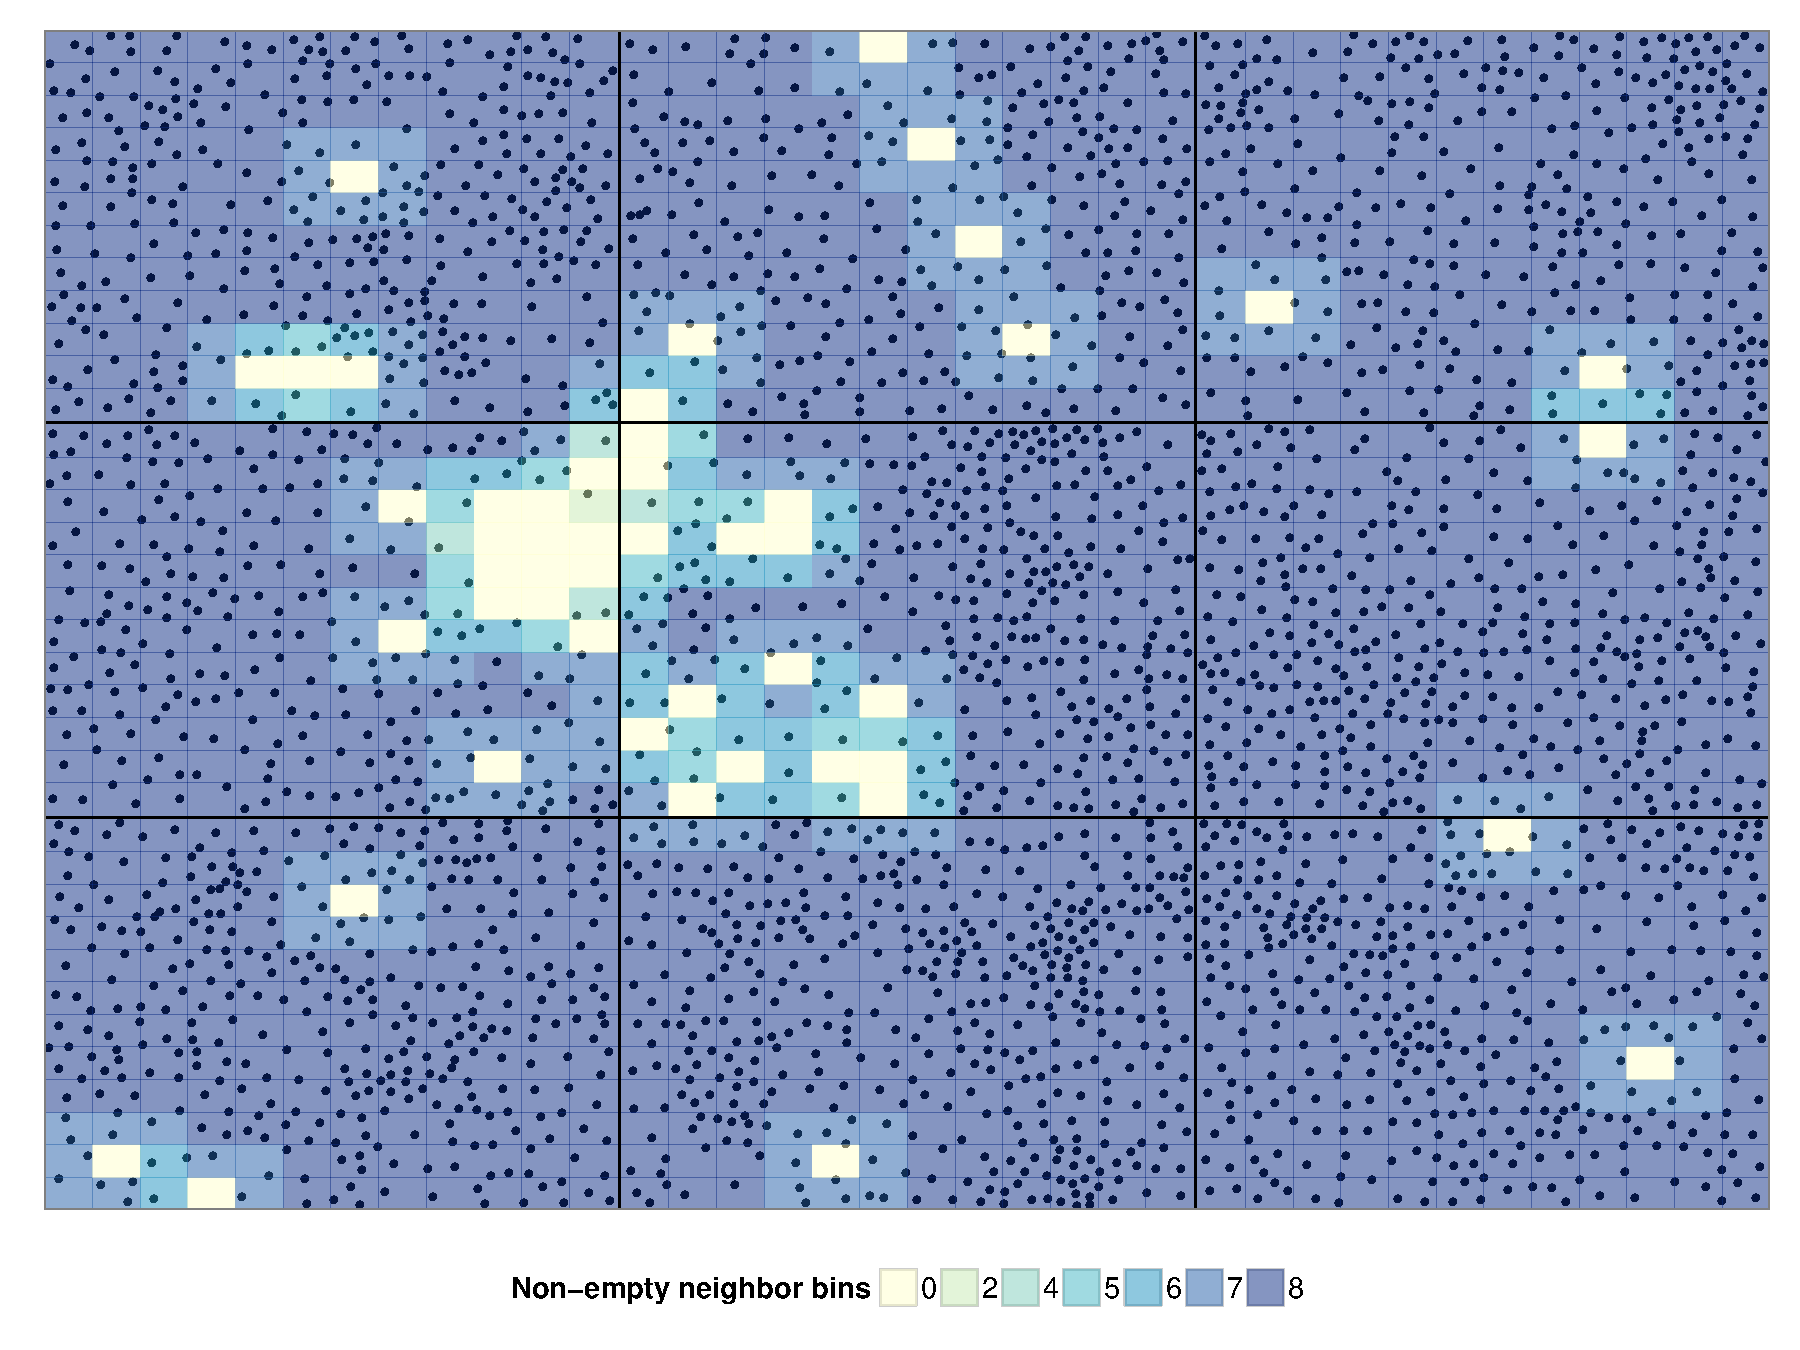
\includegraphics[width=\maxwidth]{figures/R/scf-intro/plot-scf-intro_plot-1} \caption[Visualization of cell colony edge detection by 2D binning.]{Cell colony edges are detected by 2D binning of cell center locations. Dots represent cell centers within the well H6 of plate J107-2C. Each of the nine images is segmented into 12 horizontal and 12 vertical sections yielding 144 tiles (1296 bins for the entire well). The tiles are colored according to the number of non-empty neighboring bins.}\label{fig:scf-intro_plot}
\end{figure}


\end{knitrout}



\newcommand{\knitrScfBenchmarkFacetMean}{\SI{7.77}{\milli\second}}
\newcommand{\knitrScfBenchmarkFacetSd}{\SI{2.69}{\milli\second}}
\newcommand{\knitrScfBenchmarkFacetTotal}{\SI{2.98} s}
\newcommand{\knitrScfBenchmarkEdgeMean}{\SI{515.85}{\milli\second}}
\newcommand{\knitrScfBenchmarkEdgeSd}{\SI{14.66}{\milli\second}}
\newcommand{\knitrScfBenchmarkEdgeTotal}{\SI{198.08}{\second}}
\newcommand{\knitrScfBenchmarkSpeedup}{66}


Times for my version are mean \knitrScfBenchmarkFacetMean\ (with sd \knitrScfBenchmarkFacetSd) and total runtime for a plate is \knitrScfBenchmarkFacetTotal, while theirs runs with mean \knitrScfBenchmarkEdgeMean\ (sd \knitrScfBenchmarkEdgeSd) and for a plate \knitrScfBenchmarkEdgeTotal.